\chapter{Report}
\section{a}
The Relationships between Discharge and $\Delta S$ is shown in \autoref{fig:relationship}.
\begin{figure}[htpb]\centering
	\subfigure[]{
		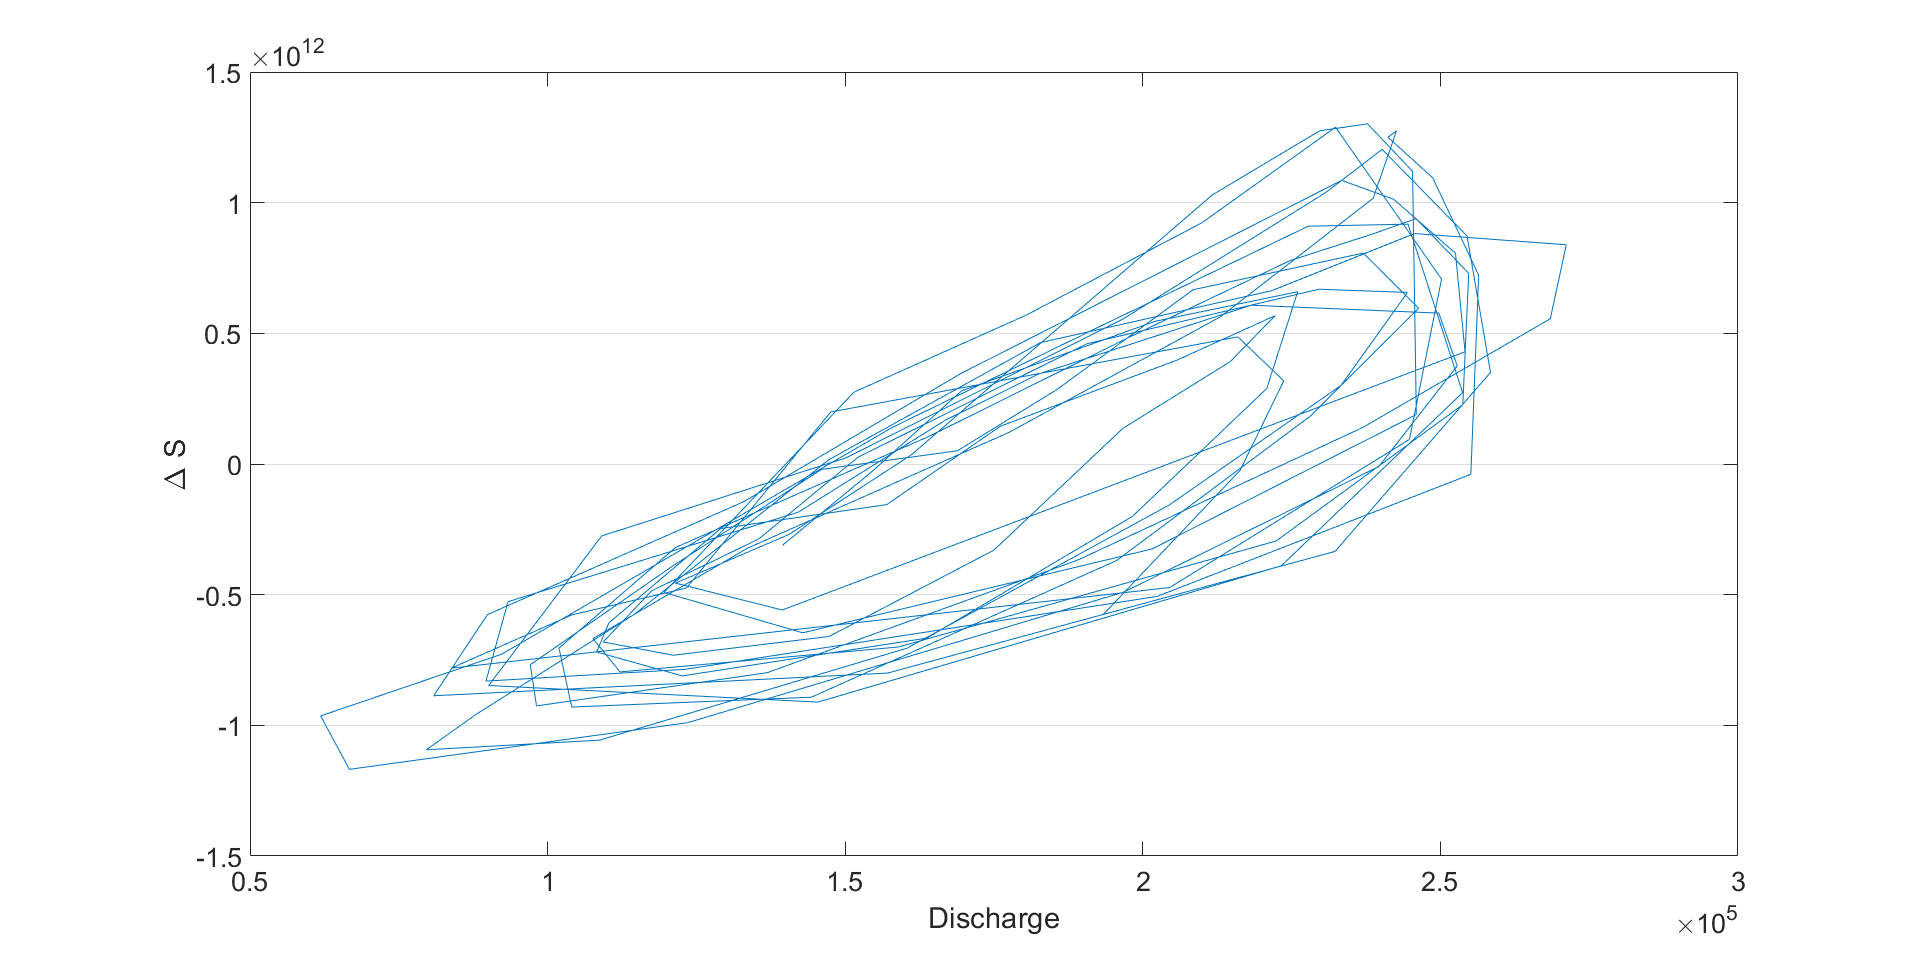
\includegraphics[width=0.9\textwidth]{relationship.png}}
	\caption{relationship between discharge and total water storage anomaly, the units are $\ut{m^3}$ in y axis and $\ut{m^3/s}$ in x axis}
	\label{fig:relationship}
\end{figure}
This indicates a linear relationship between discharge and time shifted storage anomaly. 
\section{b}
\begin{gather*}
	\frac{dR}{dt} + \frac{R}{\tau} = \omega^2_n (\Delta S + S_{0})
\end{gather*}
where $\tau$ is a hydraulic time constant
\section{c}
If we take $\Delta t$ as 1 unit, this ODE can be discretized.
\begin{gather*}
	R(t_{n+1}) = R(t_{n}) e^{\frac{\Delta t}{\tau}} + \bar{S}(t_{n}) \cdot \omega^2 \tau (e^{\frac{\Delta t}{\tau}} - 1) \\
	R(t_{n+1}) = R(t_{n}) e^{\frac{\Delta t}{\tau}} + \left(S_0 + \Delta S(t_{n})\right) \cdot \omega^2 \tau (e^{\frac{\Delta t}{\tau}} - 1) \\
	R(t_{n+1}) = \alpha R(t_{n}) + \beta  \Delta S(t_{n}) + \gamma
\end{gather*}
\section{d}
Using least square or total least square, $\alpha$, $\beta$, $\gamma$ can be calculated and so are $S_0$, $\omega$ and $\tau$. In this job, $\tau=0.3912 \ut{month^{-1}}$, $\omega = 0.2048 \ut{month^{-1}}$ and $S_0=2.18 \cdot 10^{12}\ut{m^3}$ which are not accurate. 

\section{Part 2}
The GRACE data are from JPL from 2003 to 2020 while the precipitation and evapotranspiration from 2003 to 2019. 
\begin{gather*}
	d \begin{bmatrix}
		\Delta S\\
		R
	\end{bmatrix} = \begin{bmatrix}
	0 & -1 \\
	\omega^2 & -\frac{1}{\tau}
\end{bmatrix} \begin{bmatrix}
\Delta S\\
R
\end{bmatrix} + \begin{bmatrix}
0 & 1 & -1 \\
\omega^2 & 0 & 0
\end{bmatrix} \begin{bmatrix}
S_{0}\\
P\\
ET
\end{bmatrix} \\
\begin{bmatrix}
	\Delta S_{measured} \\
	R_{measured}
\end{bmatrix} = \begin{bmatrix}
1 & 0 \\
0 & 1
\end{bmatrix} \begin{bmatrix}
\Delta S_{estimate} \\
R_{estimate} 
\end{bmatrix} 
\end{gather*}
Or $R_{measured} = R_{estimate}$ when there is no TWSA data.
\begin{gather*}
		d \begin{bmatrix}
		\Delta S\\
		R
	\end{bmatrix} = A\begin{bmatrix}
	\Delta S\\
	R
\end{bmatrix} + B \begin{bmatrix}
S_{0}\\
P\\
ET
\end{bmatrix} \\
\begin{bmatrix}
	\Delta S_{measured} \\
	R_{measured}
\end{bmatrix} = C \begin{bmatrix}
	\Delta S_{predict} \\
	R_{predict} 
\end{bmatrix} 
\end{gather*}
To discretize this state model:
\begin{gather*}
	\bm{A}_d = e^{\bm{A} \Delta t} \\
	\bm{B}_d = \bm{A}^{-1}\left(\bm{A}_d-\bm{I}\right)\bm{B} \\
	\bm{C}_d = \bm{C}
\end{gather*}
So that 
\begin{gather*}
	\bm{x}_{n+1} = \bm{A}_d \bm{x}_{n}+ \bm{B}_d \bm{u} \\
	\bm{y}_n = \bm{C}_d\bm{x}_{n} 
\end{gather*}
Using given parameter $\tau=1.201 \ut{\frac{1}{month}}$, $\omega = 0.4787 \ut{\frac{1}{month}}$ and $S_0 = 1.82 \cdot 10^{12} \ut{m^3}$. The variance for The precipitation, evapotranspiration and total water storage anomaly are known, the standard deviation of discharge will be 10\% of the discharge using the rule of thumb. A Kalman filter can then be implemented, the result are shown in \autoref{fig:kalman}
\begin{figure}[htpb]\centering
	\subfigure[]{
		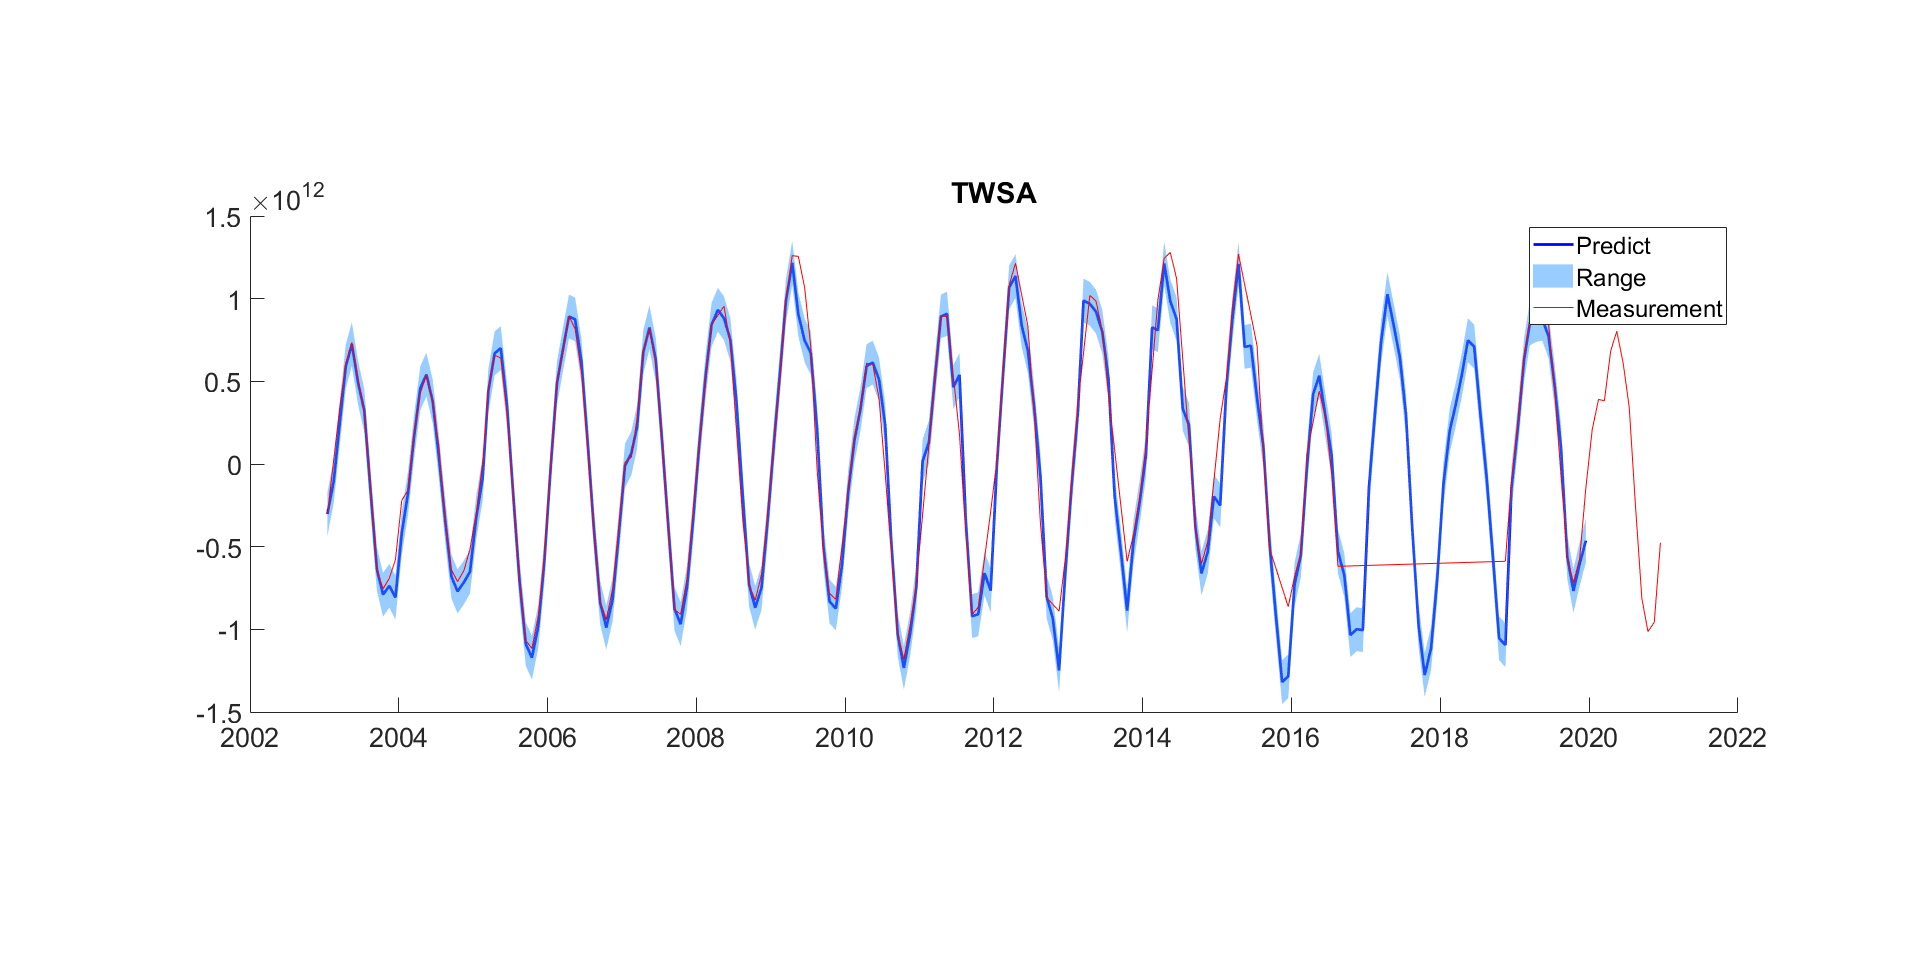
\includegraphics[width=0.9\textwidth]{TWSA.png}}
	\subfigure[]{
		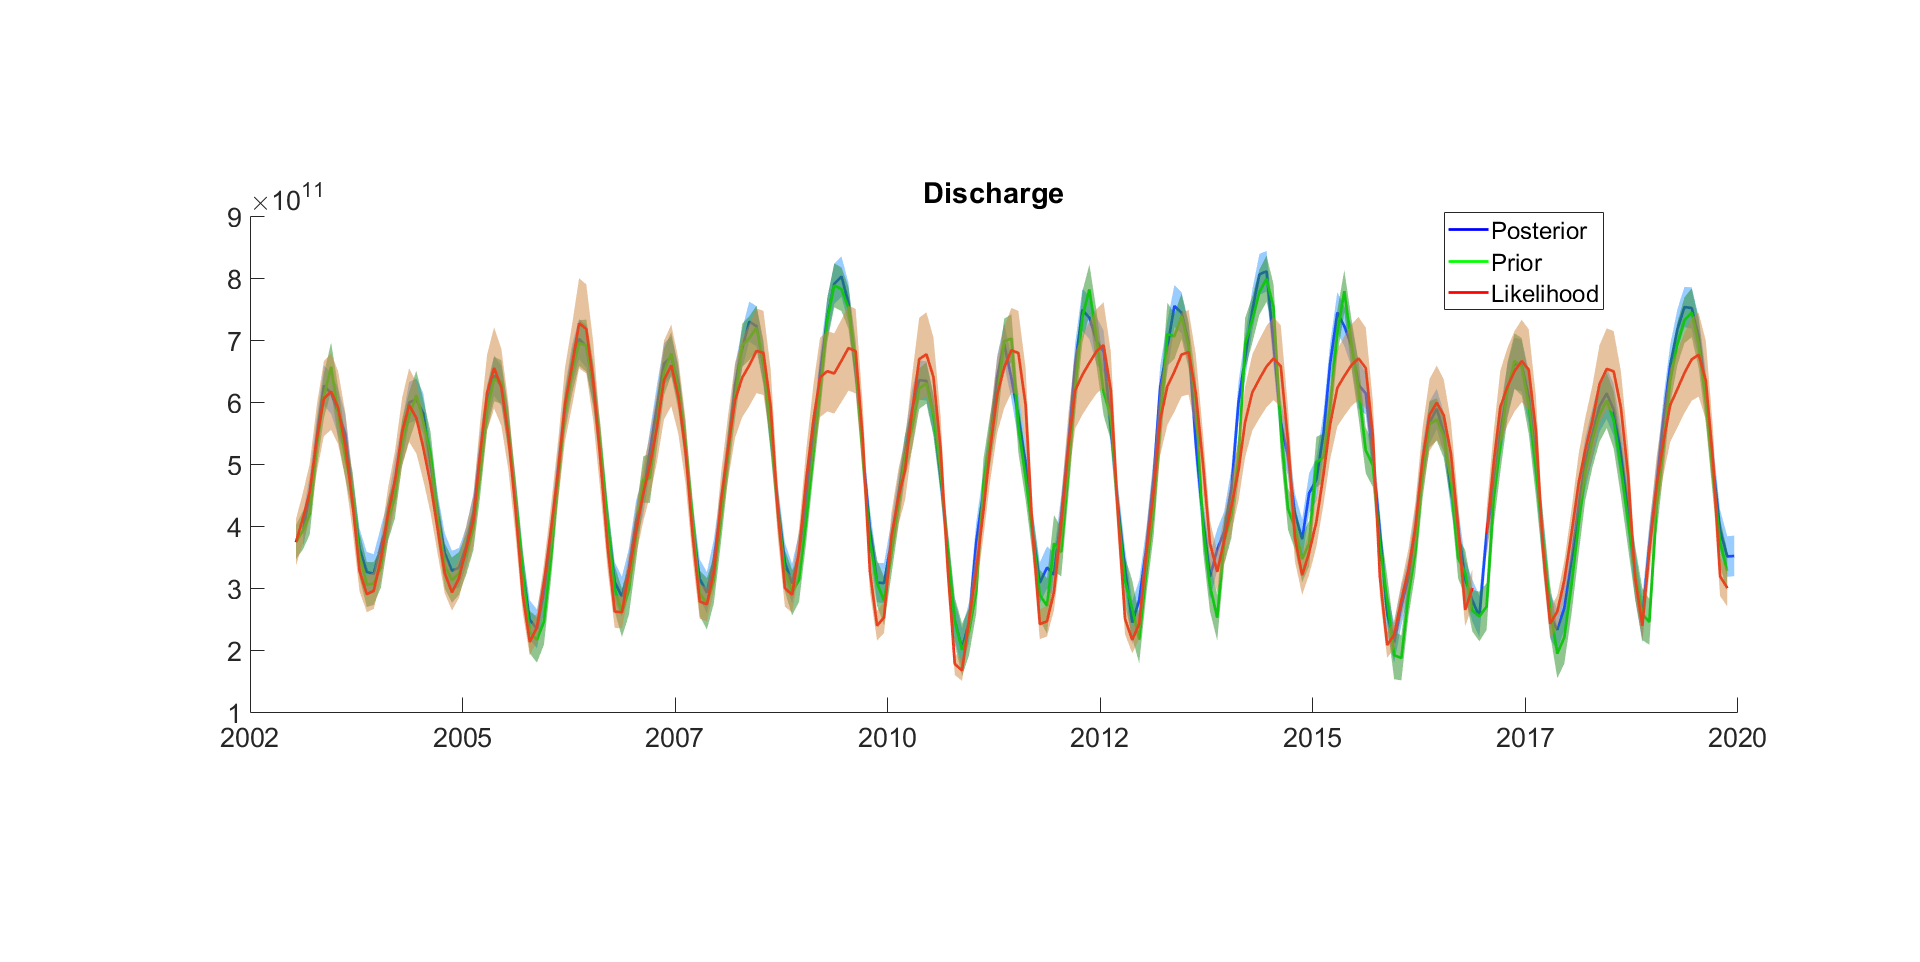
\includegraphics[width=0.9\textwidth]{R.png}}
	\caption{Kalman filter result}
	\label{fig:kalman}
\end{figure}